\documentclass[11pt]{article}
\usepackage{fullpage,amsmath,amsthm,amssymb,amsfonts,url}
\usepackage{tikz}
\usetikzlibrary{automata,positioning,arrows.meta,svg.path}

\newcommand{\emptystr}{\varepsilon}
\newcommand{\myand}{{\;\mathrel{\&}\;}}
\newcommand{\tx}[1]{\text{#1}}
\renewcommand{\t}[1]{\texttt{#1}}
\newcommand{\tuple}[1]{{\langle{#1}\rangle}}
\newcommand{\syg}{\mathord{>}}
\newcommand{\sye}{\mathord{=}}
\newcommand{\syp}{\mathord{+}}
\newcommand{\sym}{\mathord{-}}
\newcommand{\step}{\;\vdash\;}
\newcommand{\sign}{\mathord{\textit{sign}}}

\theoremstyle{definition}
\newtheorem{definition}{Definition}

\title{CSCE 355, Spring 2026\\
Programming Assignment}

\author{Due Thursday April 16, 2026 at 11:30pm EDT}

\date{}

\begin{document}

\maketitle

For the programming portion of the course (15\% of your total grade) you are to implement an interpreter for a certain kind of two-counter automaton (\textbf{2-CA}, described below).  Your program will
\begin{enumerate}
\item
read from a text file on the command line a description of a $2$-CA $A$, which is given by a sequence of transitions, one per line, then
\item
read a sequence of strings from standard input, one per line, outputting for each string $w$,
\begin{itemize}
\item
a complete computational trace of $A$ on input $w$,
\item
an indication of whether $A$ accepts or rejects $w$.
\end{itemize}
All output is to standard output.  (Standard input is from the keyboard by default but can be redirected from a file by the shell.  Standard output is to the terminal screen by default but can be redirected to a file by the shell.)
\end{enumerate}

Download and unzip the archive \url{prog-proj4.zip}.  It includes a working executable solution \t{2ca} (that runs on the linux lab machines) and a subdirectory \t{test} with some sample $2$-CAs.

\section{What is a 2-CA?}

A $2$-CA, or more generally a $k$-CA for $k\ge 1$, is analogous to a PDA with empty stack acceptance, but instead of having access to a stack, it has access to $k$ many \emph{counters}, each of which can hold a natural number at any given time (initially zero).  You will only implement the kind of $k$-CA where $k=2$.  The $k$-CA reads the input string from left to right as usual, and each transition can only depend on the current state, the currently scanned input symbol, and for each counter, \emph{whether or not it is currently zero}.  The action performed by a transition includes (possibly) changing state, consuming the scanned input symbol (or not, for $\emptystr$-transitions) and for each counter, either incrementing it, decrementing it (if nonzero), or leaving it unchanged.  The $k$-CA runs until no transitions are possible.  At that point, it accepts if the entire input is consumed and all counters are zero; otherwise, it rejects.

For example, the following $1$-CA recognizes $\{\t a^n\t b^n : n\ge 0\}$:
\begin{center}
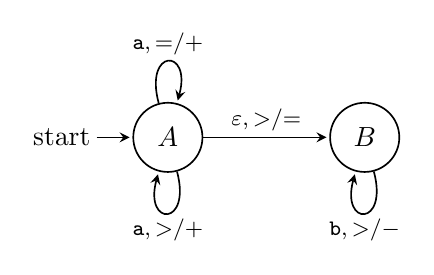
\begin{tikzpicture} [->,>=stealth,shorten >=1pt,auto,%
node distance=2.5cm,on grid,semithick,inner sep=2pt,bend angle=40]
%\draw[help lines] (0,0) grid (6,4);
\node[state,initial] (A) {$A$};
\node[state]         (B) [right=of A] {$B$};
\path [every node/.style={font=\footnotesize}]
(A)  edge [loop above] node         {$\t a,\sye/\syp$} (A)
     edge [loop below] node         {$\t a,\syg/\syp$} (A)
     edge              node         {$\emptystr,\syg/\sye$} (B)
(B)  edge [loop below] node         {$\t b,\syg/\sym$}  (B)
;
\end{tikzpicture}
\end{center}
In each transition, the slash (/) separates the condition (left) from the action (right).  So,
\begin{itemize}
\item
$\t a,\sye/\syp$ means, ``if the next input symbol is $\t a$ and the counter is \emph{equal to} zero, then consume the $\t a$ and increment the counter'';
\item
$\t a,\syg/\syp$ means, ``if the next symbol is $\t a$ and the counter is \emph{greater than} zero, then consume the $\t a$ and increment the counter'';
\item
$\emptystr,\syg/\sye$ means, ``if the counter is positive, then don't consume any input and leave the counter unchanged'' (this transition is only allowed if there is no alternative non-$\emptystr$-transition);
\item
$\t b,\syg/\sym$ means, ``if the next symbol is $\t b$ and the counter is positive, then consume the $\t b$ and decrement the counter''.
\end{itemize}

\subsection{Formalities}

If the explanation above is reasonably clear to you, you may lightly skim this section at first, referring back to it to resolve any detailed questions you may have.

There are many different and inequivalent ways to define a $k$-CA\@.  We define a very simple one here, which is \emph{deterministic}.  As usual, we let $\emptystr$ denote the empty string, and for alphabet $\Sigma$, we define $\Sigma^? := \Sigma \cup \{\emptystr\}$.

\begin{definition}
For integer $k\ge 1$, a \emph{$k$-counter automaton ($k$-CA)} is a tuple $\tuple{Q,\Sigma,\delta,q_0}$ where
\begin{itemize}
\item
$Q$ is a finite set (the \emph{state set}),
\item
$\Sigma$ is an alphabet (the \emph{input alphabet}),
\item
$q_0\in Q$ (the \emph{start state}), and
\item
$\delta : Q \times \Sigma^? \times \{\sye,\syg\}^k  \rightarrow Q \times \{\syp,\sye,\sym\}^k$ is a partial function (the \emph{transition function}).
\end{itemize}
\end{definition}

As an argument to $\delta$, the symbol ``$\sye$'' indicates the corresponding counter is currently zero, and ``$\syg$'' indicates the counter is currently positive (i.e., $>0$).  In the output of $\delta$, the symbol ``$\syp$'' means increment, ``$\sye$'' means leave unchanged, and ``$\sym$'' means decrement (but don't change the counter if it is already zero).

Here are examples where $k=2$.  For some $q\in Q$ and $a\in\Sigma$, suppose
\[ \delta(q,a,\sye,\syg) = (r,\syp,\sym) \]
for some $r\in Q$.  This means:
\begin{quote}
``If the current state is $q$, the head is scanning $a$, the first counter is zero, and the second counter is positive, then consume the $a$, go to state $r$, increment the first counter and decrement the second counter.''
\end{quote}
If
\[ \delta(q,\emptystr,\mathord{>},\mathord{>}) = (r,\mathord{=},\mathord{=}), \]
this means:
\begin{quote}
``If the current state is $q$ and both counters are positive, then without consuming an input symbol go to state $r$, leaving both counters unchanged.''
\end{quote}
It is possible during a computation that an $\emptystr$-transition and a non-$\emptystr$-transition are both available at the same time.  To ensure deterministic behavior, we impose the following ``greedy'' rule:
\begin{quote}
An $\emptystr$-transition should be taken \textbf{only} if there is no legal non-$\emptystr$-transition available.
\end{quote}

To define behavior formally, we limit ourselves to $2$-CAs.  (The definition generalizes to $k$-CAs in the obvious way.)

\begin{definition}\label{def:2ca}
Let $A := \tuple{Q,\Sigma,\delta,q_0}$ be a $2$-CA\@.  An \emph{instantaneous description (ID)} or \emph{configuration} of $A$ is a $4$-tuple $(q,x,n_1,n_2)$, where $q\in Q$, \ $x\in\Sigma^*$, and $n_1,n_2$ are natural numbers (nonnegative integers).

Given a string $w\in\Sigma^*$, the \emph{initial configuration of $A$ on input $w$} is $(q_0,w,0,0)$ (start state, entire input unread, both counters zero).

A configuration $(q,x,n_1,n_2)$ is \emph{accepting} if and only if $x = \emptystr$ and $n_1 = n_2 = 0$.  Any other configuration is \emph{rejecting}.  (The state $q$ can be arbitrary).
\end{definition}

Similar to the case of PDAs, the ID $(q,x,n_1,n_2)$ means,
\begin{quote}
``The current state is $q$, the unconsumed portion of the input is $x$, and the two counter values are $n_1$ and $n_2$, respectively.''
\end{quote}

Next we define one step of a computation as a \emph{partial} successor function on IDs.  (A partial function is one that is not necessarily defined on all arguments.)  The next definition will make this easier.

\begin{definition}
For a natural number $n$, define
\[ \sign(n) := \begin{cases}
\syg & \mbox{if $n>0$,} \\
\sye & \mbox{if $n=0$.}
\end{cases} \]
Define
\begin{align*}
\Delta(\sym) &:= -1, & \Delta(\sye) &:= 0, & \Delta(\syp) &:= 1.
\end{align*}
\end{definition}

Let $A$ be as in Definition~\ref{def:2ca}.  Given a state $q\in Q$, a string $w\in\Sigma^*$, and natural numbers $n_1,n_2$, the \emph{successor} of the configuration $C := (q,w,n_1,n_2)$ (if it exists) is the configuration defined by the following rules (letting $s_1 := \sign(n_1)$ and $s_2 := \sign(n_2)$):
\begin{itemize}
\item
If $w=ax$ for some $a\in\Sigma$ and $x\in\Sigma^*$, then
\begin{itemize}
\item
if $\delta(q,a,s_1,s_2) = (r,t_1,t_2)$ where $r\in Q$ and $t_1,t_2\in\{\sym,\sye,\syp\}$, then the successor of $C$ is $(r,\; x,\;\max\{0,\,n_1+\Delta(t_1)\},\;\max\{0,\,n_2+\Delta(t_2)\})$;
\item
if $\delta(q,a,s_1,s_2)$ is undefined but $\delta(q,\emptystr,s_1,s_2) = (r,t_1,t_2)$, then the successor of $C$ is $(r,\; w,\;\max\{0,\,n_1+\Delta(t_1)\},\max\{0,\,n_2+\Delta(t_2)\})$;
\item
if both $\delta(q,a,s_1,s_2)$ and $\delta(q,\emptystr,s_1,s_2)$ are undefined, then $C$ has no successor.
\end{itemize}
\item
If $w = \emptystr$, then
\begin{itemize}
\item
if $\delta(q,\emptystr,s_1,s_2) = (r,t_1,t_2)$ where $r\in Q$ and $t_1,t_2\in\{\sym,\sye,\syp\}$, then the successor of $C$ is $(r,\;\emptystr,\;\max\{0,\,n_1+\Delta(t_1)\},\max\{0,\,n_2+\Delta(t_2)\})$;
\item
if $\delta(q,\emptystr,s_1,s_2)$ is undefined, then $C$ has no successor.
\end{itemize}
\end{itemize}
For IDs $C_1$ and $C_2$, we write, ``$C_1\step C_2$'' to mean that $C_2$ is the successor of $C_1$.

A \emph{computation path} of $A$ on input $w\in\Sigma^*$ is a sequence $C_0\step C_1\step \cdots$ of IDs starting with the initial configuration where each subsequent ID is the successor of the previous one.  The path ends when it reaches a configuration with no successor.  If the last configuration is accepting, then $A$ \emph{accepts} $w$; if the last configuration is rejecting, then $A$ \emph{rejects} $w$.  Note that it is possible that the path never ends; in this case, we say that $A$ \emph{loops} on $w$.

The \emph{language recognized by $A$} is defined as you would expect:
\[ L(A) := \{ w\in\Sigma^* : \mbox{$A$ accepts $w$} \}. \]
(By this definition, if $A$ loops on $w$, then $w\notin L(A)$.)

\subsection{Example}
Consider the $1$-CA given by the transition diagram above.
\begin{itemize}
\item
On input $\t{aabb}$, the computation path is
\[ (A,\t{aabb},0) \step (A,\t{abb},1) \step (A,\t{bb},2) \step (B,\t{bb},2) \step (B,\t b,1) \step (B,\emptystr,0) \;\;\;\mbox{(accept)} \]
\item
On input $\t{aab}$, the computation path is
\[ (A,\t{aab},0) \step (A,\t{ab},1) \step (A,\t{b},2) \step (B,\t{b},2) \step (B,\emptystr,1) \;\;\;\mbox{(reject)} \]
\item
On input $\t{abb}$, the computation path is
\[ (A,\t{abb},0) \step (A,\t{bb},1) \step (B,\t{bb},1) \step (B,\t b,0)\;\;\;\mbox{(reject)} \]
\item
On input $\t{bbaa}$, the computation path is
\[ (A,\t{bbaa},0) \;\;\;\mbox{(reject)} \]
\item
On input $\emptystr$, the computation path is
\[ (A,\emptystr,0) \;\;\;\mbox{(accept)} \]
\end{itemize}

(By the way, a $1$-CA can be easily simulated by a PDA where the size of the stack is used for the counter.  Thus $1$-CAs can only recognize context-free languages.  This is not true for $2$-CAs, however; some of the $2$-CAs in the test files recognize non-context-free languages.)

\section{Input File Format}

Your program takes a filename (a text file with the description of a $2$-CA) as the only command line argument.  The file contains a list of the allowed transitions, one per line.  A transition has the following syntax:
\begin{verbatim}
(<from_state>,<symbol?>,<c1_cond>,<c2_cond>) -> (<to_state>,<c1_action>,<c2_action>)
\end{verbatim}
The arguments to the transition function are to the left of the arrow, and the action to be performed is to the right.  Items surrounded by angle brackets are not meant literally but instead are meant to be substituted for various syntactic elements:
\begin{itemize}
\item
\t{<from\_state>} and \t{<to\_state>} are state labels---the state transitioning from and to, respectively.  Each consists of a pound sign (``\t\#'') followed by any string of zero or more alphanumeric characters.  The underscore (\verb+_+) counts as an alphanumeric character.  \emph{The pound sign by itself denotes the start state.}
\item
\t{<symbol?>} is either a single character (the next character to be consumed, which could be any printable character except a space, tab, or newline), or nothing (indicating an $\emptystr$-transition).
\item
\t{<c1\_cond>} and \t{<c2\_cond>} are the conditions on counters~1 and 2, respectively.  Each is either ``\t{=}'' (meaning equal to zero), ``\t{>}'' (meaning greater than zero), or ``\t{*}'' (a wildcard meaning any value; see below).
\item
\t{<c1\_action>} and \t{<c2\_action>} are the actions to be performed on counters~1 and 2, respectively.  Each is either ``\t{+}'' (increment), ``\t{=}'' (leave unchanged), or ``\t{-}'' (decrement).
\end{itemize}
All spaces and tabs in a line containing a transition should be ignored.  Any occurrence of \t{//} indicates the start of a comment (running to the end of the line) and should be ignored.  Empty lines must be commented.

There will always be at least one transition out of the start state (\t{\#}), but transitions can appear in any order within the file.

\subsection{Example}

The $1$-CA given in Section~1 above is given in the file \t{ab.txt} in the \t{test} subdirectory (with different state labels and two counters):
\begin{verbatim}
// 2-CA to recognize the language { a^nb^n : n >= 0 }
//
// The 2nd counter is unused and stays 0 the whole time.
//
(#,       a,*,=) -> (#,+,=)         // Read an "a" and increment counter 1
(#,        ,>,=) -> (#read_bs,=,=)  // epsilon-transition from # to #read_bs
(#read_bs,b,>,=) -> (#read_bs,-,=)  // Read a "b" and decrement counter 1
\end{verbatim}
The second transition is an $\emptystr$-transition, as there is no non-whitespace character in the 2nd argument.  The star (\t{*}) used in the first transition is a wildcard.  That line is shorthand for two separate transitions:
\begin{verbatim}
    (#,a,=,=) -> (#,+,=)
    (#,a,>,=) -> (#,+,=)
\end{verbatim}

\section{Simulation}

After you read in a $2$-CA from the file and internalize it, your program then reads a sequence of input strings from standard input, one per line, ending with an end-of-file marker (ctrl-D if typing from the linux keyboard).  For each input string, you simulate the $2$-CA on that string, writing to standard output the computation path, one ID per line, then saying either ``ACCEPT'' or ``REJECT'' at the end as appropriate.

Each input string will be at most 128 characters in length.

\section{How to Test Your Code}

The zip file package includes an executable solution \t{2ca} that runs on the linux lab machines.\footnote{The solution does two things that you are \emph{not} required to do: it checks for syntax and semantic errors in the $2$-CA file (all test files we give you are error-free).}  It has a verbose option that makes the interaction more user-friendly.

In a linux terminal shell in the directory into which you unzipped the file, type
\begin{verbatim}
    ./2ca --verbose test/ab.txt
\end{verbatim}
You should first see an internalized description of the $2$-CA, followed by a prompt to enter a string.  Enter any string of \t a's and \t b's and you'll see a complete computation path on that input string followed by whether the string was accepted or rejected.  (To enter $\emptystr$ as the input, just hit RETURN.)  You can use ``\t{-v}'' instead of ``\t{--verbose}'' to turn this option on.

Without the verbose option, you'll see no description of the $2$-CA, nor any explicit prompt for a string, nor the column headers on the computation path.  {\bf Your program should match the behavior of \t{2ca} \emph{without} the verbose option.}  You don't have to line things up neatly in columns, because we will ignore spaces and tabs in your output.

You should test your program in place of \t{2ca} on this and the other \t{*.txt} files in the \t{test} directory and compare the outputs with those given by \t{2ca}.

\section{How Your Program is Graded}

The grading of your work will be automated via a script running on linux.
%(These scripts are found from the project homepage: \url{https://cse.sc.edu/~fenner/csce355/prog-proj2/sp25/index.html}).
Therefore we are requiring you to stick to a simple, uniform interface for your program:  Your program must be able to be run via a simple command-line invocation on one of the linux boxes in the department's linux lab, and all I/O will be ASCII text.  You may write your program in any programming language you want, provided it is implemented on the linux machines in the CSCE linux lab.
% (We recommend Java or C or C++ or Perl or Python or Ruby or ML or Haskell or Prolog or Scheme or \ldots.)
To repeat: your program (after compiling, if necessary) should be a stand-alone executable that can be run directly from the linux \t{bash} shell, requiring no special user interface to execute (e.g., Eclipse).\footnote{It's OK if we need to invoke the JVM by preceding your main class name with ``java'' on the command line, or the python interpreter by preceding your program with ``python3''.}  More about this below.

\subsection{What the script does}

%This assignment is not meant to be overly taxing or time-consuming.
%Most of the time spent will probably be to get the input read in correctly.

%The \t{diff} utility in linux is very useful for this.
Let's say you have a stand-alone executable called \t{my\_interpreter}.
%\footnote{If your code is invoked by feeding it to, say, \t{python3} or \t{java}, then you will have a way of indicating this; see the \t{build-run.txt} description below.}
Then the script effectively does the following for the test file \t{ab.txt}:
\begin{verbatim}
$ ./my_interpreter test/ab.txt < test/ab.in | ./sw.pl > tmp1.txt
$ ./2ca test/ab.txt < test/ab.in | ./sw.pl > tmp2.txt
$ diff tmp1.txt tmp2.txt
\end{verbatim}
If \t{tmp1.txt} and \t{tmp2.txt} are identical, then \t{diff} quits with no output, which indicates that your program ran correctly.  Otherwise, \t{diff} returns a list of discrepancies between the two files, line by line.  The program \t{sw.pl} is a Perl script that strips whitespace (spaces and tabs) from each line of standard input and sends the results to standard output.  It also strips carriage returns (\verb+\r+) which are included with files produced on DOS/Windows.  Our grading script will repeat the above for each $2$-CA in the test directory, collecting the outputs of the \t{diff} commands into a file \t{comments.txt} that also includes scoring information.

You can run the above commands yourself if you want more clarity on how we will grade you.  If the symbols ``\t{<}'', ``\t{|}'', and ``\t{>}'' above are unfamiliar to you, you should read up on input/output redirection and pipes in linux.

%Do the above for each $2$-CA described in the test directory.

You may assume that when we test your program for grading, the $2$-CA descriptions will adhere to their respective formats, i.e., you won't need to error-check the files.  You can send anything you want to standard error; the grading program will ignore it.\footnote{We call the three I/O streams open by default on GNU/Linux programs \emph{standard input} (keyboard input by default), \emph{standard output} (screen output by default), and \emph{standard error} (unbuffered output sent to the screen by default, even if standard input and output are redirected by the system).  Some programming environments may use different names for these streams, e.g., C programs using \t{stdio.h} for high-level I/O call these \t{stdin}, \t{stdout}, and \t{stderr}, respectively; C++ programs typically use \t{cin}, \t{cout}, and \t{cerr} for the same purpose.}

\subsection{Style}

Your code should be economically written, well-structured, and well-commented, following the common stylistic guidelines of the programming language you use.  The code should also be reasonably efficient, but this is a secondary requirement.  The script allows a generous 11 seconds for each run of your code.  You'll be fine as long as your runs keep to this time limit; otherwise, you won't get credit for that run.

%\section{Testing and Grading}
\subsection{Summary}

As we mentioned, your project will be graded automatically.  To grade your project, we will use a script and the test files we have provided to test and grade your project.  Just to be perfectly clear: we will grade your project by running a script on it with owner privileges using one of the linux lab machines.  We will not run your code personally.  The comments produced by that script will determine your grade.  This means that you will not get credit for attempting to do something.  You will only get credit for what actually works, as determined by the script run on a CSE linux Lab machine.

We will test your code on seven different $2$-CAs.  Each $2$-CA corresponds to two files in the \t{test} directory: the \t{.txt} file contains the $2$-CA's description, and the \t{.in} file contains the input strings for the simulation.  You earn 15 points for every $2$-CA your program handles correctly, except for \t{match\_delim2.txt}, which is worth 20 points.  Any incorrect behavior (including time-out) earns zero points for that $2$-CA\@.  Your score will not exceed 100 points.

\section{How to Submit}

Submission will be via Blackboard.  Upload a single file, either a .zip file or a .tar.gz file, containing
\begin{enumerate}
\item
all your source code files, which should all be in the same directory, i.e., no subdirectories (and no automatically generated files, please),
\item
an optional file \t{readme.txt} with anything you want to tell us (we will read this with our own eyes at our discretion), and
\item
a file \t{build-run.txt} giving linux (\t{bash}) shell commands to compile and/or run your program.  Don't include the command line arguments (e.g., \t{test/ab.txt}); we will supply those separately when we run your program.  This file should be named \t{build-run.txt} and placed in the same directory as your other source files.  See below for the contents of this file.
\end{enumerate}

IMPORTANT NOTE:  You \emph{must} use either the ZIP format (file extension .zip) or the GZIPPED TAR format (file extension .tar.gz) for your submission file.  Your file will be de-archived either with \t{unzip} or with \t{gunzip; tar -xf}, depending on your file name's extension.  Do not use any other archive format, particularly the RAR format, which is proprietary to Windows (I personally do not have Windows on any machine I use).  If you deviate from the allowed formats, you risk getting zero credit for the entire assignment.  Keep in mind that linux file names are case-sensitive.

\subsection{Examples of build-run files}

Suppose you implement your program in Java, and your main class is called \t{MyInterpreter}.  Then your \t{build-run.txt} file would look like this:
\begin{verbatim}
# Lines like these are comments and will be ignored
Build:
  javac MyInterpreter.java
Run:
  java MyInterpreter
# Don't include command line arguments to the run command!
# The indenting is optional.
\end{verbatim}
For another example, suppose you implement your program in C as a single compilation unit called \t{my\_interpreter.c}.  Then your \t{build-run.txt} file would look something like this:
\begin{verbatim}
Build:
  gcc my_interpreter.c
  mv a.out my_interpreter
Run:
  ./my_interpreter
# Again, no command line arguments, please.  They will be supplied automatically.
\end{verbatim}
Note that you can have any number of build commands, and they will be executed in order (in the directory containing your source files) before the run command.  Always give the Build commands first before the Run command.

Suppose instead that you have several compilation units for your programs, including shared code, and a complicated build procedure, but you have a single \t{Makefile} controlling it all, capable of producing an executable called \t{my\_interpreter}.  Then the \t{build-run.txt} file can just look something like this:
\begin{verbatim}
Build:
  make -B
Run:
  ./my_interpreter
\end{verbatim}
(Use the \verb|-B| option or \verb|--always-make| option with \t{make}; it will build your entire program from source regardless of any intermediate files.)

As a final example, suppose you implement your program in Python, which is a scripting language that can be run directly without a compilation step.  Then your \t{build-run.txt} file might look like this:
\begin{verbatim}
Build:
Run:
  python3 my_interpreter.py
# You still need to say "Build:" even though there are no build commands.
# For the linux machines you should use python3 instead of python.
\end{verbatim}

\iffalse
\subsection{A Windows vs.\ Linux pitfall}

Windows-based text files end each line with the two-character sequence \verb+\r\n+ (carriage return, newline), and GNU/linux/Mac OSX and similar systems expect only an \verb+\n+ ending each line.  We strongly recommend against doing your development on a Windows box, but if you absolutely must, be aware that your program may not work properly with the test script if they are copied over without newline conversion.  (This is the cause of many mysterious failures when running the test script.)  Our Linux boxes support the \t{scc} command.  Running
\begin{verbatim}
    scc my_text_file.txt
\end{verbatim}
converts all \verb+\r\n+ sequences to \verb+\n+ in \t{my\_text\_file.txt}.  (Note that this command alters the contents of the file and does \emph{not} produce a backup copy.)
\fi

\section{Two Common Pitfalls}

No allowances will be made for falling for either of these:

\begin{description}
\item[Not testing your code on a lab machine.]
You tested your code on your laptop and it ran perfectly, so you just submitted without bothering to test it on one of the linux lab machines.  You're then shocked to see that you got a zero for the entire assignment.  This happens more often than you'd think.  Even if your laptop is running linux, it may be configured differently from the machines in the lab.  In the labs, you need to use \t{python3} to invoke Python.
\item[Windows Versus Linux.]  In text files created in DOS/Windows, a newline is given by two-character sequence: carriage-return/linefeed (in C-like languages, the code is \verb+\r\n+.  GNU/Linux systems only use the linefeed character to indicate a new line.  The test files are all GNU/Linux-created.  Make sure your parser is not expecting carriage-returns (\verb+\r+) in the test files.
\end{description}

The moral is not to wait until the last hour, or even the last day, to test your code on a linux lab machine.

\section{Do Your Own Work}

The code you write and submit must not come from another person or persons, even in part.  You may discuss the homework with others at the conceptual level (see the next paragraph), but you may not copy code either directly or indirectly from any other human source, even if you modify it afterwards.  Likewise, you must take all reasonable precautions not to let your code be copied by anyone else, either in this class or in future classes.  This includes uploading or developing your code on a web platform---such as SourceForge or GitHub---in a way that can be seen by others.  Violating this policy constitutes a violation of the Carolina Honor Code, and will have serious consequences, including, but not limited to, failure of the course.

Discussing the project with others in the class is allowed (even encouraged), but you must include in your \t{readme.txt} file the names of those with whom you discussed the project.

\subsection{Use of AI}

You \emph{are} allowed make use of AI for this project without penalty, \t{but} if you do, you \emph{must} include in your \t{readme.txt} file what resource(s) you used and the specific queries you made to that resource.  Failing to do so constitutes violation of class policy and the Carolina Honor Code, with the same consequences as given above.

Please note that this means you must retain the text of your queries for inclusion in the \t{readme.txt} file.

\subsection{Ask}

If you have any questions about what this policy means, please review the relevant section of the course syllabus or ask me.

\end{document}
